\documentclass[10pt]{beamer}
\usetheme[
%%% option passed to the outer theme
%    progressstyle=fixedCircCnt,   % fixedCircCnt, movingCircCnt (moving is deault)
  ]{DNA}
\usepackage{natbib}
\usepackage{float}
\usepackage{graphicx}
\usepackage[labelformat=empty,font=scriptsize,skip=0pt,justification=justified,singlelinecheck=false]{caption}
\usepackage[caption=false]{subfig}
\usepackage{amsmath}
\usepackage{mathtools}
\usepackage[percent]{overpic}
\usepackage{tikz}
\usetikzlibrary{arrows}
\usepackage{ulem}
\usepackage{multimedia}
\usepackage{siunitx}
\DeclareSIUnit\basepair{bp}

%remove the icon
\setbeamertemplate{bibliography item}{}

%remove line breaks
\setbeamertemplate{bibliography entry title}{}
\setbeamertemplate{bibliography entry location}{}
\setbeamertemplate{bibliography entry note}{}

%\setbeameroption{hide notes} % Only slides
%\setbeameroption{show only notes} % Only notes
% \setbeameroption{show notes on second screen=right} % Both

% Give a slight yellow tint to the notes page
\setbeamertemplate{note page}{\pagecolor{yellow!5}\insertnote}\usepackage{palatino}

% If you want to change the colors of the various elements in the theme, edit and uncomment the following lines

% Change the bar colors:
%\setbeamercolor{DNA}{fg=red!20,bg=red}

% Change the color of the structural elements:
%\setbeamercolor{structure}{fg=red}

% Change the frame title text color:
%\setbeamercolor{frametitle}{fg=blue}

% Change the normal text color background:
%\setbeamercolor{normal text}{fg=black,bg=gray!10}

% % beamer: How to place images behind text (z-order)
% % (http://tex.stackexchange.com/a/134311)
% \makeatletter
% \newbox\@backgroundblock
% \newenvironment{backgroundblock}[2]{%
%   \global\setbox\@backgroundblock=\vbox\bgroup%
%     \unvbox\@backgroundblock%
%     \vbox to0pt\bgroup\vskip#2\hbox to0pt\bgroup\hskip#1\relax%
% }{\egroup\egroup\egroup}
% \addtobeamertemplate{background}{\box\@backgroundblock}{}
% \makeatother

%-------------------------------------------------------
% INCLUDE PACKAGES
%-------------------------------------------------------

\usepackage[utf8]{inputenc}
\usepackage[english]{babel}
\usepackage[T1]{fontenc}
\usepackage{helvet}

%-------------------------------------------------------
% DEFFINING AND REDEFINING COMMANDS
%-------------------------------------------------------

% colored hyperlinks
\newcommand{\chref}[2]{%
  \href{#1}{{\usebeamercolor[bg]{DNA}#2}}
}

%-------------------------------------------------------
% INFORMATION IN THE TITLE PAGE
%-------------------------------------------------------

\title[] % [] is optional - is placed on the bottom of the sidebar on every slide
{% is placed on the title page
      \textbf{Nucleosome Heterogeneity Governs Chromatin Organization}
}

\subtitle[Nucleosome Heterogeneity]
{%
      \textbf{2018--12--04}
}
% \author[Bruno Beltran]{Trent Newman$^{1}$, \textbf{Bruno Beltran$^{2}$}, James McGehee$^{1}$,
% Cori Cahoon$^{1}$, Dan Elnatan$^{1}$, Dan Chu$^{1}$, Andrew Spakowitz$^{2}$,
% Sean Burgess$^{1}$ \\
% \ttfamily brunobeltran0@gmail.com}
% \institute[UC Davis Mol \& Cell Bio and Stanford Biophysics]{$^{1}$Department of
% Molecular and Cellular Biology, UC Davis \\ $^{2}$Department of Biophysics,
% Stanford University}

\author[Bruno Beltran]
{Bruno Beltran \\
{\ttfamily brunobeltran0@gmail.com}
}

\institute[]
{%
    Graduate Student, Spakowitz Lab\\
    Biophysics PhD Program, Stanford University

  %there must be an empty line above this line - otherwise some unwanted space is added between the university and the country (I do not know why:( )
}

% \date{February 18, 2018}

%-------------------------------------------------------
% THE BODY OF THE PRESENTATION
%-------------------------------------------------------

\begin{document}

%-------------------------------------------------------
% THE TITLEPAGE
%-------------------------------------------------------

{\1% % this is the name of the PDF file for the background
\begin{frame}[plain,noframenumbering] % the plain option removes the header from the title page, noframenumbering removes the numbering of this frame only
    \titlepage{} % call the title page information from above
\end{frame}}

% \begin{frame}{Content}{}
% \tableofcontents
% \end{frame}

\begin{frame}{Big Picture}
    \includegraphics[width=0.21\linewidth]{./2018-12-04-090226_878x1113_scrot.png}
    \includegraphics[width=0.21\linewidth]{./2018-12-04-090240_876x1102_scrot.png}
    \includegraphics[width=0.21\linewidth]{./2018-12-04-090256_875x1122_scrot.png}
    \includegraphics[width=0.21\linewidth]{./2018-12-04-090316_874x1120_scrot.png}
    \includegraphics[width=0.21\linewidth]{./2018-12-04-090355_874x1119_scrot.png}
\end{frame}

%-------------------------------------------------------
    \section{Introduction}
%-------------------------------------------------------

\begin{frame}{Chromatin}
    \begin{center}
        \includegraphics[height=0.60\textheight]{./qual-figures/chromemt-zoom.jpg}

        \tiny{Ou, H.D. et al.\@ \textit{ChromEMT:\@ Visualizing 3D chromatin
        structure and compaction in interphase and mitotic cells}. Science 357 (2017).}
        \note[item]{Define chromatin.}
    \end{center}
\end{frame}

\begin{frame}{Modeling Chromatin}
    \begin{center}
        \only<1>{\includegraphics[height=0.60\textheight]{./qual-figures/model-detail-slide-1.png}}
        \only<2>{\includegraphics[height=0.60\textheight]{./qual-figures/model-detail-slide-2.png}}
        \only<3>{\includegraphics[height=0.60\textheight]{./qual-figures/model-detail-slide-3.png}}
        \only<4>{\includegraphics[height=0.60\textheight]{./qual-figures/model-detail-slide-4.png}}
    \end{center}

    \only<2->{\tiny{Ou, H.D. et al.\@ \textit{ChromEMT:\@ Visualizing 3D chromatin
    structure and compaction in interphase and mitotic cells}. Science 357
    (2017).}}

    \only<3->{\tiny{Quinn MacPherson (unpublished data)}}
\end{frame}

%-------------------------------------------------------
    \section{Results}
%-------------------------------------------------------

\begin{frame}{Figure 1}
\begin{figure}[t]
    \centering
    \subfloat[]{\label{fig:entry-exit}
        \begin{overpic}[width=100pt]{./paper-figures/fig-1a-nucleosome-geometry.png}
            \put(16,-3){\large$\displaystyle\theta$}
            \put(10,59){\large$\displaystyle\Omega_\text{entry}$}
            \put(62,17.5){\large$\displaystyle\Omega_\text{exit}$}
        \end{overpic}%
    }\hspace{2em}
    \subfloat[]{\label{fig:linker-effect}
        \begin{overpic}[width=130pt]{./paper-figures/fig-1b-helicity-effect.png}
            \put(17,11){\parbox{1.5cm}{\centering DNA Helicity}}
            \put(-2,47){\large$\displaystyle\phi$}
            \put(-6,63){$\displaystyle\SI{33}{\basepair}$}
            \put(11,77){$\displaystyle-\SI{2}{\basepair}$}
            \put(40,81){$\displaystyle\SI{35}{\basepair}$}
            \put(61,72){$\displaystyle+\SI{2}{\basepair}$}
            \put(76,46.5){$\displaystyle\SI{37}{\basepair}$}
        \end{overpic}
    }%
\end{figure}
\end{frame}

\begin{frame}{Figure 2}
\begin{figure}
    \centering
    \mbox{\includegraphics[scale=1.4]{../../deepti/nuc_chain_tmp/plots/PRL/fig2a_r2_homogenous_vs_wlc-scaled.pdf}
    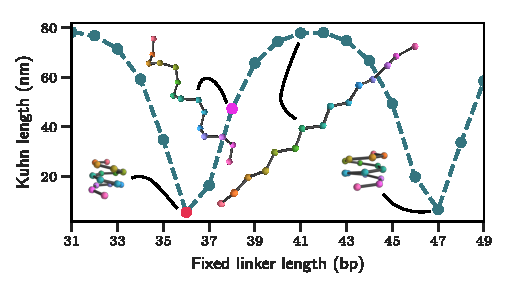
\includegraphics[scale=1.4]{../../deepti/nuc_chain_tmp/plots/PRL/fig2b_kuhn_length_in_nm_31to51links_0unwraps-with-renderings.pdf}}
\end{figure}
\end{frame}

\begin{frame}{Figure 3}
    \centering
    \includegraphics[height=0.75\textheight]{../../deepti/nuc_chain_tmp/plots/PRL/fig-3-kuhn_length_vs_window_size_41_sigma0to40-v4.pdf}
\end{frame}

\begin{frame}{Figure 4}
\begin{figure}
    \centering
    \mbox{\includegraphics[scale=1.4]{../../deepti/nuc_chain_tmp/plots/PRL/fig4a_r2_exp_vs_wlc-scaled.pdf}
    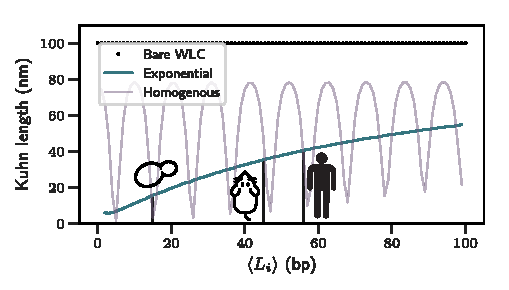
\includegraphics[scale=1.4]{../../deepti/nuc_chain_tmp/plots/PRL/fig4b_kuhn_exponential-with-images.pdf}}
\end{figure}
\end{frame}

\begin{frame}{Figure 5}
    \begin{center}
        \includegraphics{./paper-figures/fig5_looping_hetero31to52bp_bold3curves.pdf}
    \end{center}
\end{frame}

%-------------------------------------------------------
    \section{Conclusion}
%-------------------------------------------------------

\begin{frame}{Summary}
    \begin{itemize}[<+->]
        \item On time scales longer than nucleosome turnover, chromatin is an
            effective WLC.\@
        \begin{itemize}[<+->]
            \item Nucleosome heterogeneity $\to$ structural universality
            \item Small amounts of heterogeneity are required to justify ``maximally
                entropic'' approximation.
            \item Maximum entropy picture is well approximated by an effective
                WLC.\@
        \end{itemize}
        \item On time scales shorter than nucleosome turnover, nucleosome
            spacing drastically affects chromatin organization.
    \end{itemize}
\end{frame}

% \begin{frame}[allowframebreaks]
%     \frametitle{References}
%     \bibliographystyle{amsalpha}
%     \bibliography{./multilocus.bib}
% \end{frame}

{\1
\begin{frame}[plain,noframenumbering]
  \finalpage{Thank you!}
\end{frame}}

\end{document}
